%The title of Chapter 1 shall be Introduction.  It shall justify and highlight the problem 
%posed,  define the topic and explain the aim and scope of the work presented in the thesis.  It 
%may also highlight the significant contributions from the investigation.


With widespread adoption of virtualization for hosting applications,
service providers (like Amazon EC2~\cite{ec2}) can facilitate better 
performance isolation, security and elastic resource provisioning.
A virtualization-based provisioning model is attractive for both 
providers~\cite{ec2}\textemdash{}multiplex resources among several customers, and 
clients\textemdash{}\textit{pay-per-use}, use and pay for only as much resource 
as required. Instances of both \emph{public}~\cite{ec2} and 
\emph{private}~\cite{ubuntu-private-cloud} clouds exist, 
which leverage virtual machines for flexible provisioning.

%Several issues, some of which are\textemdash{}mapping of resource requirements
%from physical to virtual environments~\cite{profiling-and-modeling},
%placement policies for virtual machines~\cite{autonomic-vm-placement},
%dynamic resource provisioning~\cite{autonomic-virtual-resource-management},
%runtime consolidation and migration~\cite{sandpiper},
%storage provisioning and access management~\cite{ip-networked-storage}
%need to be addressed to provision applications in virtual execution
%environments. Further, these problems
%need to be addressed in the context of meeting service level
%agreements and resource guarantees~\cite{managing-sla-violations},
%and simultaneously maximizing the resource multiplexing potential.
%Server consolidation and flexible resource provisioning 
%\cite{autonomic-vm-placement}, \cite{autonomic-virtual-resource-management}, 
%\cite{sandpiper}, \cite{capacity-management} are
%virtual machine migration-enabled techniques aimed to reduce provider-side
%resource sprawl and to address elastic resource requirements, respectively.

%Since application demands are expectedly continuously varying, resource
%requirements will also be correspondingly elastic. To support this,
%virtualization-based services require automated and dynamic resource
%provisioning.
%Further, if a single physical machine faces an explosion of resource
%requirements, one or more of its virtual machines may need to be
%\textit{migrated} to other physical machines for load balancing. Thus, dynamic
%resource provisioning can be both intra-PM (when physical machine or PM
%has sufficient resources to accommodate increased demands)
%and inter-PM (when PM has insufficient resources and hence
%the virtual machine or VM needs to be migrated to another lesser loaded PM).

%It is widely acknowledged~\cite{capacity-planning, emerging-research-directions}
%that the average utilization
%levels in a data-center is around 20\%, that is to say,
%the peak-to-average utilization ratios are very high. Typically,
%under periods of high load, a VM may be allocated to a single PM of its
%own, and when the load falls back down, it may be moved back to another
%non-idle PM, such that the total resource utilization needs are 
%fulfilled on the target PM, and no SLAs are breached of either the VM under
%consideration, or the VMs that were already executing on the target PM. This
%strategy, known as \textit{Server Consolidation}, 
%allows under-utilized physical machines to be switched off, 
%thereby saving power and cooling
%costs. This idea is illustrated briefly in Fig.~\ref{consolidation-migration}.

%\begin{figure}[t]
%\begin{center}
%% \noindent\makebox[\textwidth]{% 
%	\subfloat[Initially VMs colocated on single PM]{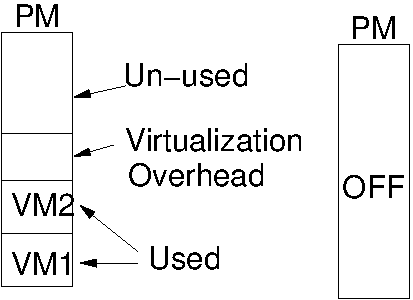
\includegraphics[scale=0.55]{presyn-figures/initially-consolidated.eps}} \hfill
%	%\subfloat[Initially VMs colocated on single PM]{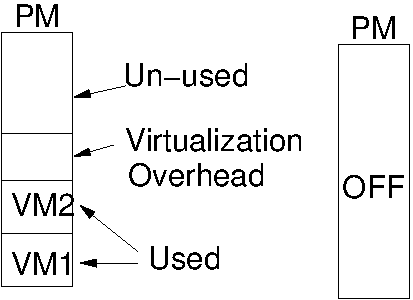
\includegraphics[scale=0.6]{presyn-figures/initially-consolidated.eps}} \hspace{0.6in}
%	%\subfloat[Slight load increase accommodated]{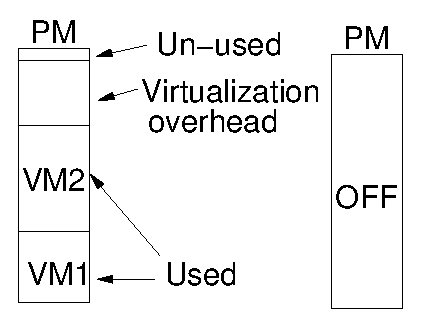
\includegraphics[scale=0.6]{presyn-figures/slight-load-increase.eps}} \\ \vspace{0.2in}
%	\subfloat[Slight load increase accommodated]{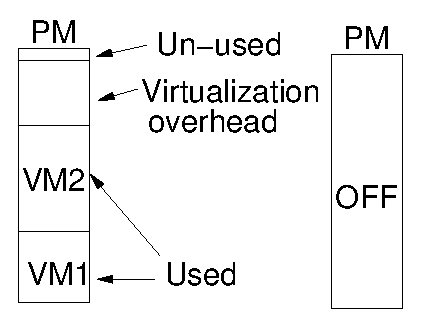
\includegraphics[scale=0.55]{presyn-figures/slight-load-increase.eps}} \hfill
%	\subfloat[Heavy load requires VM migration]{\includegraphics[scale=0.55]{presyn-figures/heavy-load-needs-migration.eps}} \hfill
%	\subfloat[Migrate back when load falls]{\includegraphics[scale=0.55]{presyn-figures/low-load-migrate-back.eps}}
%\caption{Server consolidation and migration for dynamic resource provisioning}
%\label{consolidation-migration}
%\end{center}
%\end{figure}

Virtualization enables dynamic resource allocation and quicker deployment
of services. Instead of installing new hardware for deploying a service,
virtualization allows transparent, on-demand deployment
on a few
processors in an existing multi-processor machine and avoids new machine
procurement delays. %~\cite{xen-art-of-virtualization}.
Virtualization allows accommodation of varying load-levels by
on-demand resource allocation %~\cite{xen-art-of-virtualization-revisited}
and also reduces application downtime. %~\cite{google-live-migration}.
Due to above benefits of virtualization,
many hosting centers have transitioned from providing 
Hardware as a Service (HaaS) to 
Infrastructure as a Service (IaaS) instead~\cite{ec2}.
The primary difference between HaaS and IaaS is that the
former involves use or leasing of physical
hardware/machine whereas the latter involves
leasing of virtual resources/machines.

Most web-based applications are multi-tiered and virtualization
offers the possibility of hosting each of these tiers (e.g., the 
web-server tier, the application logic tier and 
the database server) on separate virtual machines.
%elastically provisionable virtual machines. 
%Such differentiated hosting
%for various tiers is preferable 
%to hosting the entire %application as a monolithic entity 
%hosted on a single peak-provisioned %physical machine since 
%This enables independent and flexible resource management 
%of the different tiers. Additionally, due to
%elastic potential of resource allocation to virtual machines,
%differentiated hosting on virtual machines can help avoid resource
%wastage on under-utilized physical machines.
The major factors that affect the performance of a 
virtualized application are\textemdash{}available network capacity, disk access bandwidth
and virtualization overheads.
%When multi-tiered applications are instantiated in a virtual
%environment, the following major factors affect their 
%performance\textemdash{}available network capacity, disk access bandwidth
%and virtualization overheads. 
When multiple virtual machines (VMs) are placed on a single 
physical machine (PM),
they compete for various resources like CPU, memory, network and disk I/O
and interact in many conflicting ways. 
In any given virtualized environment, the physical resources available can 
be broadly categorized into the following:-

\paragraph{I. Resources allocated to the virtual machines.} 
Every virtual machine has access to a set of resources, similar
to those available on physical machines.
For example, virtual CPU, VM page cache, virtual disk, etc.
%are resources that are allocated to each virtual machine.
%These are
%usually statically allocated in today's datacenters~\cite{ec2}, 
%but can be better managed using dynamic provisioning 
%techniques~\cite{sandpiper}.

\paragraph{II. Resources in the virtualized host.} 
These are resources at the virtualized host to support and enable
virtualization.
For example, the hypervisor incurs CPU overheads
for virtualization. %~\cite{measuring-cpu-overhead}. 
The host's page cache is also used for buffering of physical I/O access,
on behalf of VMs.
\\
\\
In this thesis, we address two
important problems related to the management of both
these types of resources more efficiently, towards the overall goal
of optimizing the performance of virtualized applications and services.

\subsection*{Thesis contributions} 
\paragraph{1. Affinity-aware Modeling of CPU usage for Virtualized Applications.} 
This problem deals with managing the network 
usage of VMs and estimating CPU 
requirement on both the VM and its host PM.
Since different tiers of an application require mutual network
communication, \textit{colocation} of communicating VMs
on the same PM reduces physical network 
usage. \textit{Network affinity} is the presence of network
communication between a pair of VMs, and is 
\textit{intra-PM} when the VMs are colocated, and 
\textit{inter-PM} when they are dispersed onto different PMs.
Thus, the nature of network affinity is \textit{mutable} (i.e., changing
between inter-PM and intra-PM) upon VM migrations.
%We make the case that since there is significant change in CPU resource
%usage when the VMs are colocated versus when they are dispersed, it is
%essential to capture such changes, %via a model,
%for server consolidation and VM placement decisions.
%We define the presence of network traffic between a pair
%of VMs as their \textit{network affinity}, and state that the
%nature of this network traffic is \textit{mutable} based on
%whether the VMs are colocated or dispersed, i.e., network affinity
%can change between \textit{inter-PM} or \textit{intra-PM}
%upon VM migrations.
%can be \textit{inter-PM} or {intra-PM} based on whether the
%PMs are colocated on a single PM, or dispersed on different PMs. 
%In other words, the
%nature of the inter-VM network traffic can change between being
%intra-PM and inter-PM depending on whether the VMs are hosted
%on the same physical machine or on different physical machines.
%We explore the effect of the \textit{mutable}
%network traffic on CPU usage of colocated and dispersed VMs. More
%specifically, the question is

In our work, 
%we explore the difference in CPU utilization due
%to \textit{network affinity}, and propose models to
%estimate the changed CPU utilization.
%Specifically, 
we perform network benchmarking, which 
demonstrates effects of network affinity on CPU usage when VMs 
are colocated versus dispersed. Next, we develop VM \textit{pair-wise} models
that can estimate the ``colocated'' CPU usage, on being 
input their individual dispersed-case resource usages.
We also build similar models to estimate the ``dispersed'' CPU
usage based on the individual colocated-case resource usages.
For the ``colocation'' and ``dispersion'' models, we first 
built models that predicted the total (or absolute) CPU usage
upon migration\textemdash{}these CPU models use all resource (CPU, disk, mutable
and immutable network) usage profiles as their input. However, these models
had an error of around 4\%. So, next we built enhanced models
to predict only the difference (or differential) CPU usage\textemdash{}these
models use only the \textit{mutable} network traffic metrics as input,
and have maximum error within 2\%. Finally, we demonstrated the
application of \textit{pair-wise} models to predict for multi-VM
scenarios, with high accuracy.

\paragraph{2. Using Implicit Caching Hints for {D}isk I/O {R}eduction in Virtualized Environments.}
This problem deals with managing the cache
usage on a virtualized host to improve disk access performance 
of VMs.
Due to increased permeation of virtualization-based systems, there is a lot of
inherent content similarity in systems like email servers, web servers 
and file servers. 
%All this data resides on disk and is fetched by corresponding
%applications, as and when required. 
Harnessing content similarity can help 
avoid duplicate disk I/O requests that fetch the same content repeatedly.
In this work, we incorporate intelligent I/O redirection within the 
storage virtualization engine of the device to manage the underlying 
block-cache like a content-cache.

We build a disk read-access optimization called DRIVE, that
identifies content similarity across multiple blocks, and performs
hint-based read I/O redirection.
% than other systems.
A metadata store is maintained and implicit caching hints are collected 
based on the VM's disk accesses.
Using the hints, read I/O redirection is performed from within the VM's virtual
block device, to manipulate the entire
host-cache as a content-deduplicated cache.
Our trace-based evaluation using a custom simulator, reveals that
DRIVE achieves up to 20\% better cache-hit ratios and reduces
up to 80\% disk reads. It also achieves up to 
97\% content deduplication in the host-cache.

% \section{Thesis contributions}
